\documentclass[11pt]{article}
\usepackage[margin=1in]{geometry}
\usepackage{amsmath}
\usepackage{booktabs}
\usepackage{graphicx}
\usepackage{subcaption}
\usepackage{hyperref}

\title{Time Series Forecasting Project Report}
\author{Group ID: TODO \\ Members: TODO}
\date{}

\begin{document}
\maketitle

\begin{abstract}
TODO: Briefly summarize the forecasting problem, your method, and your main validation result.
\end{abstract}

\section{Introduction}
TODO: Describe the forecasting task and why it is interesting.

\section{Related Work}
TODO: Discuss relevant forecasting models and cite them, e.g., Transformers, TCNs, RNNs, state-space models, or other methods you used.

\section{Method}
TODO: Describe your model architecture, input representation, loss, training procedure, and important design choices. Include a figure if useful.

\section{Experiments}
TODO: Report validation results, compare against the naive last-value and seasonal mean baselines, and include ablations or analysis.

\begin{table}[h]
\centering
\begin{tabular}{lrr}
\toprule
Method & Validation Metric & Notes \\
\midrule
Naive last-value baseline & TODO & minimum baseline \\
Seasonal mean baseline & TODO & stronger reference \\
Our model & TODO & TODO \\
\bottomrule
\end{tabular}
\caption{Validation results. Lower is better for all listed metrics.}
\end{table}

\section{Conclusion}
TODO: Summarize findings, limitations, and possible future work.

\section*{Contributions}
TODO: State each group member's contribution.

\section*{Appendix}

\begin{figure}[p]
    \centering
    \begin{subfigure}[t]{0.40\linewidth}
        \centering
        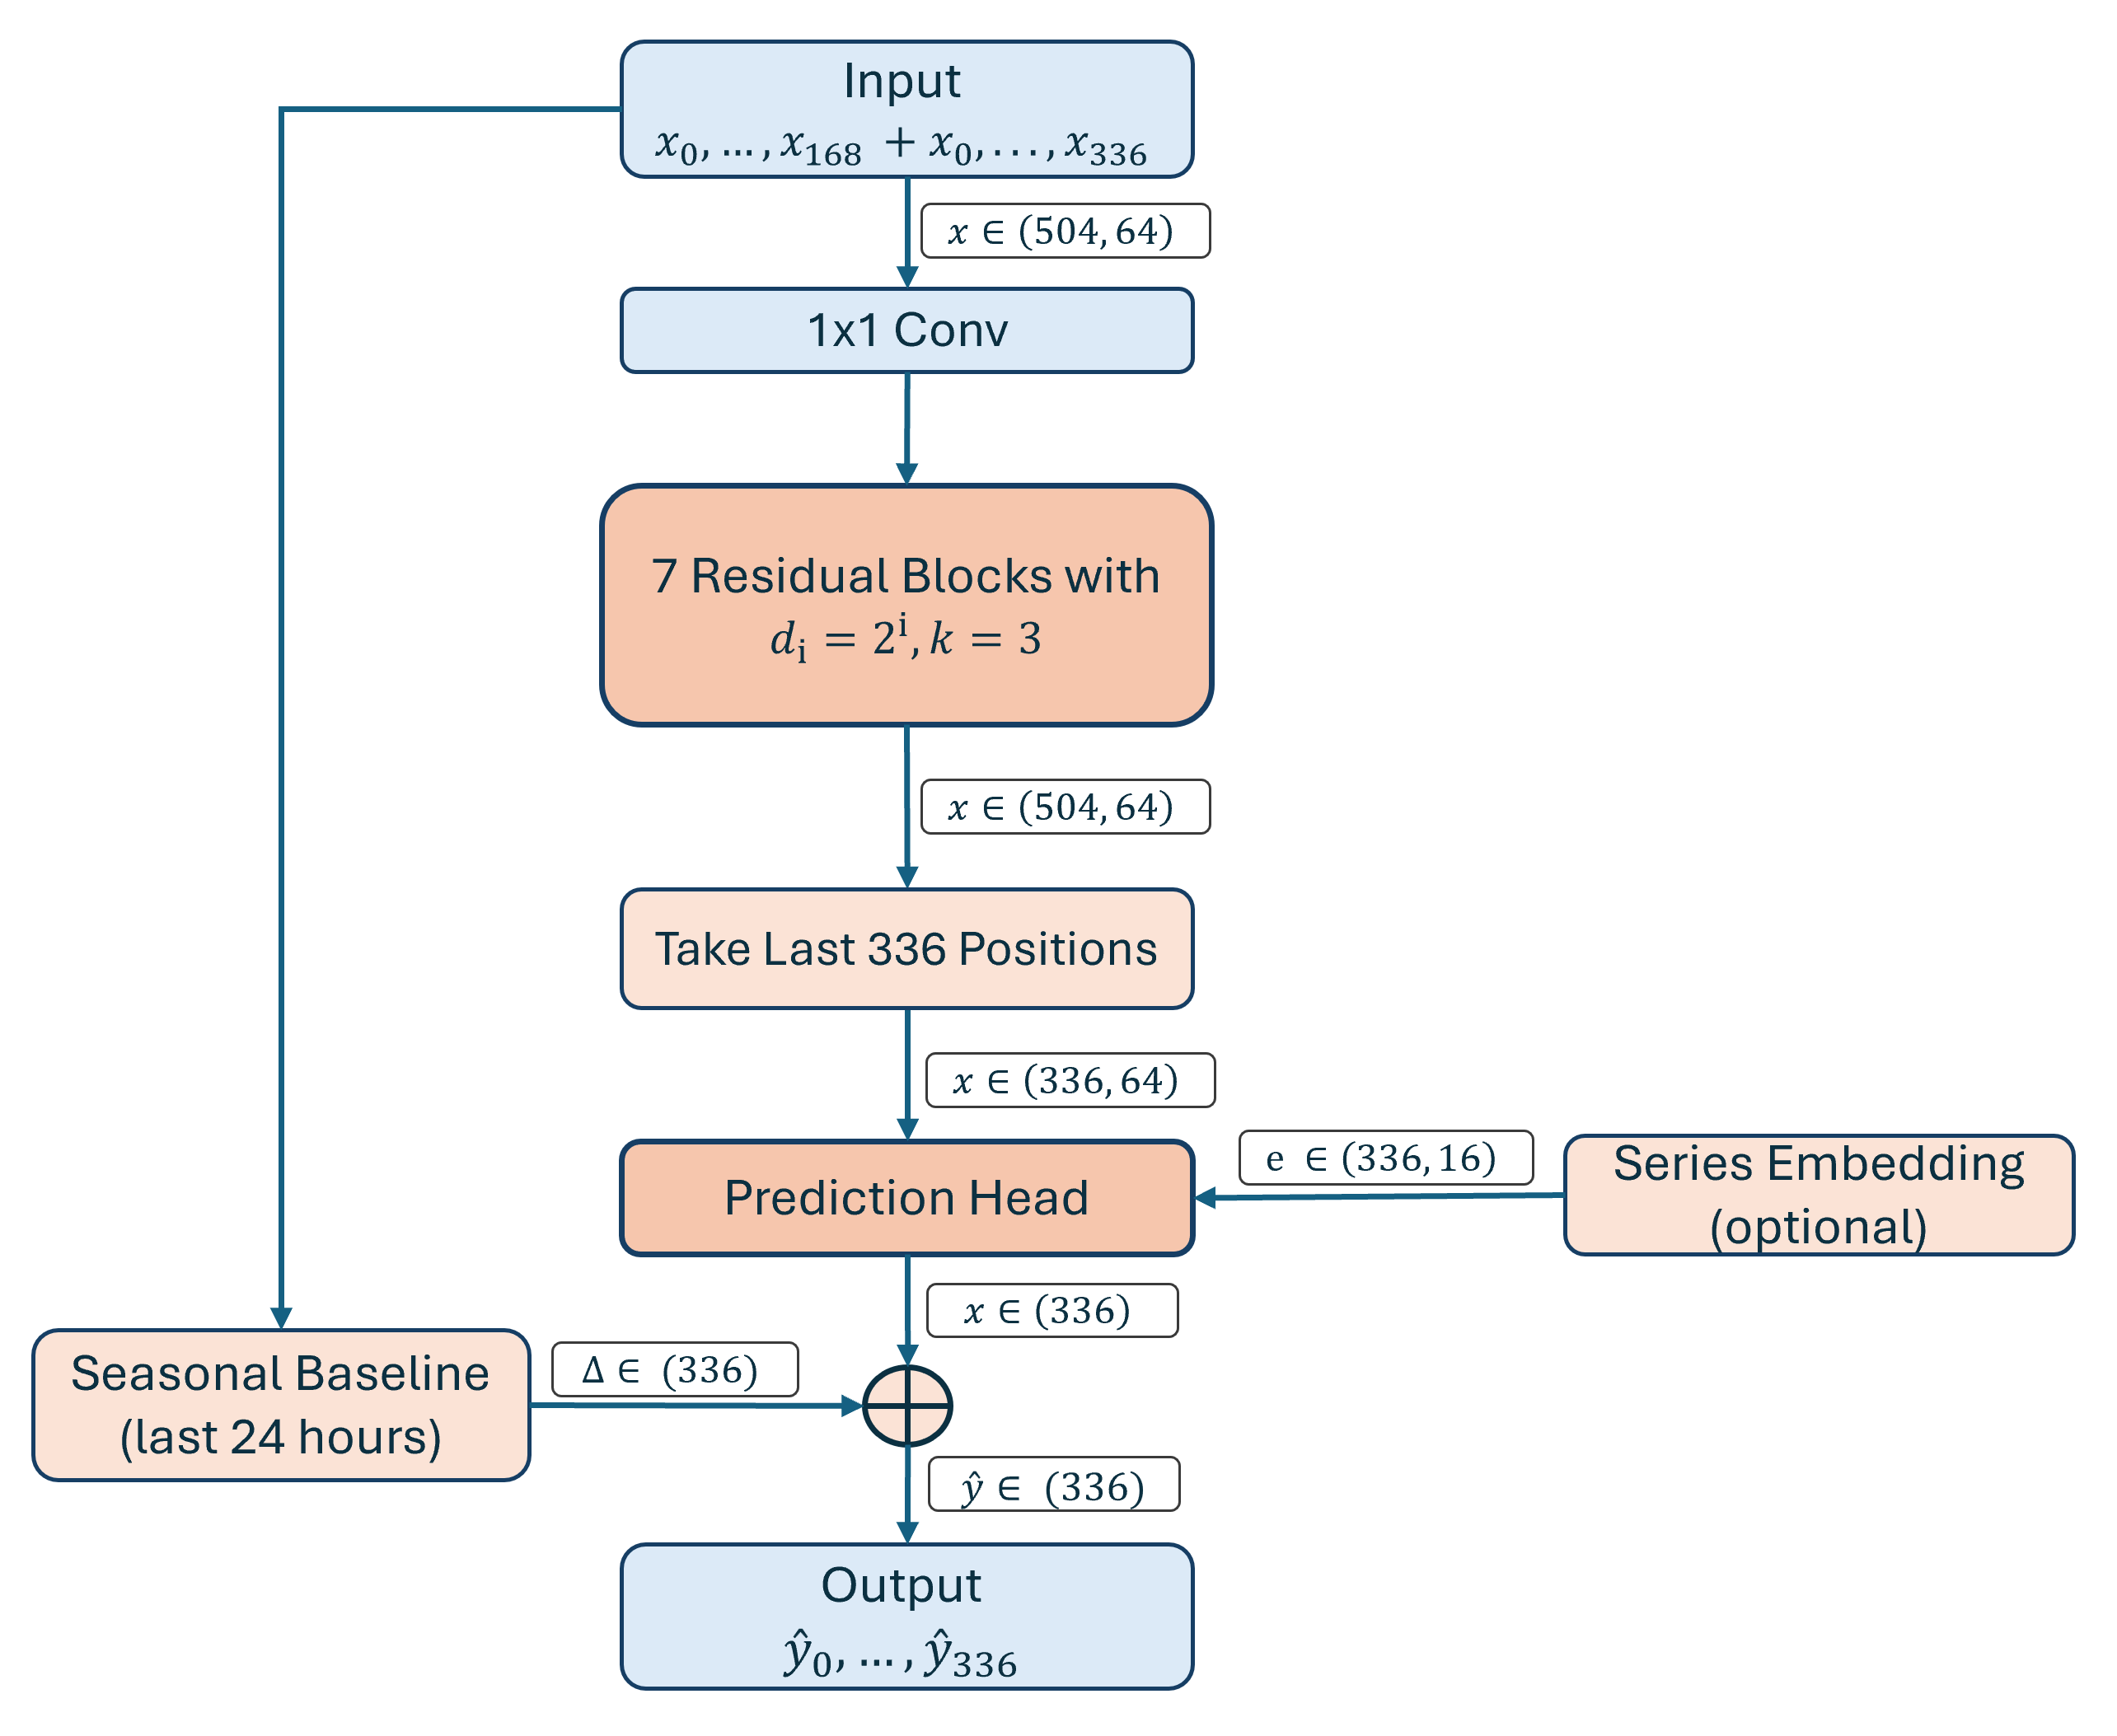
\includegraphics[width=\linewidth,height=0.52\textheight,keepaspectratio]{../../figures/tcn_diagram.png}
        \caption{End-to-end TCN forecasting architecture.}
        \label{fig:tcn-overview}
    \end{subfigure}\hfill
    \begin{subfigure}[t]{0.24\linewidth}
        \centering
        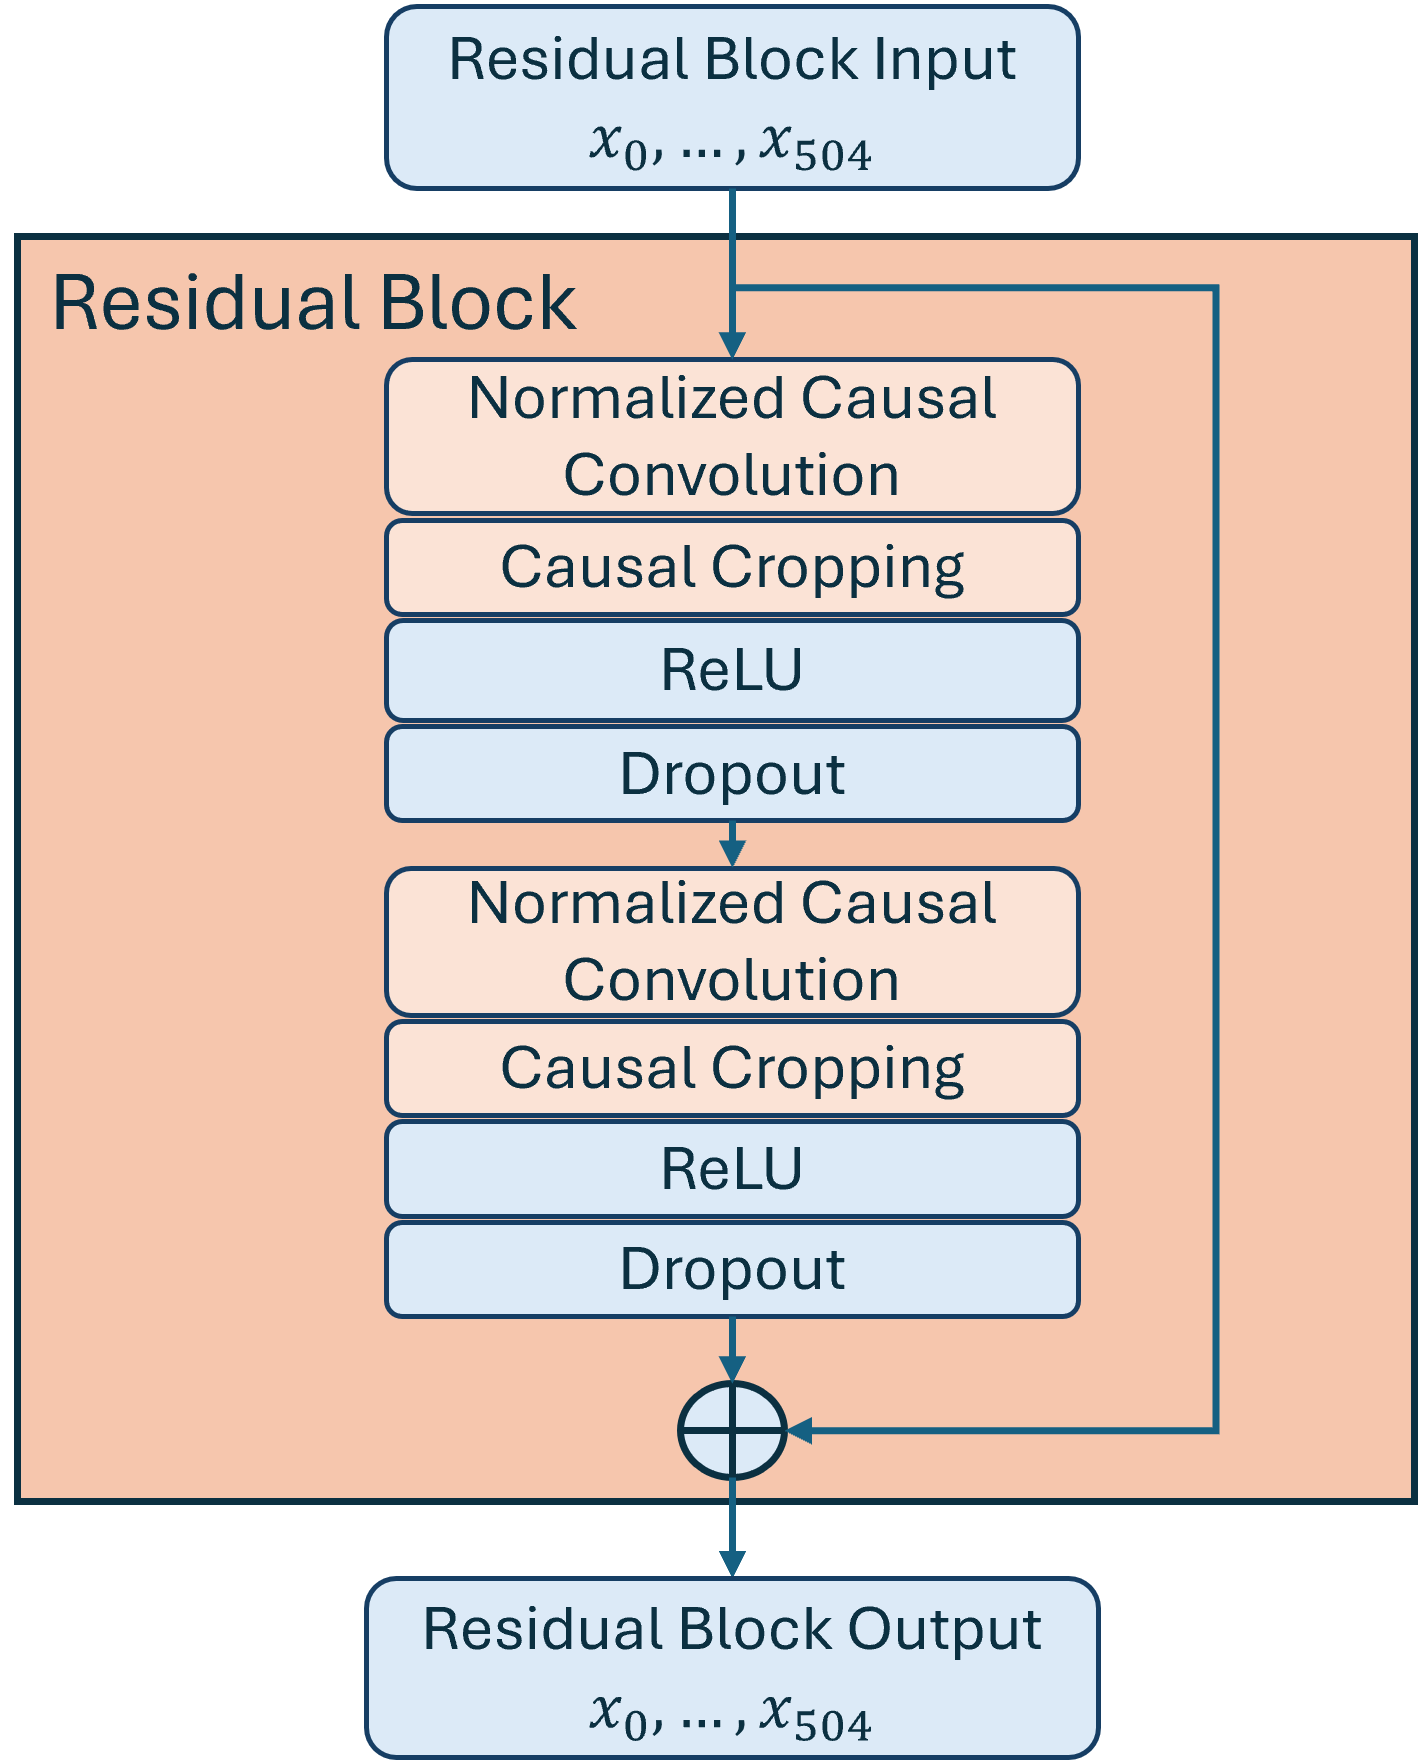
\includegraphics[width=\linewidth,height=0.52\textheight,keepaspectratio]{../../figures/res_block_tcn.png}
        \caption{Internal structure of one residual block.}
        \label{fig:tcn-residual-block}
    \end{subfigure}\hfill
    \begin{subfigure}[t]{0.32\linewidth}
        \centering
        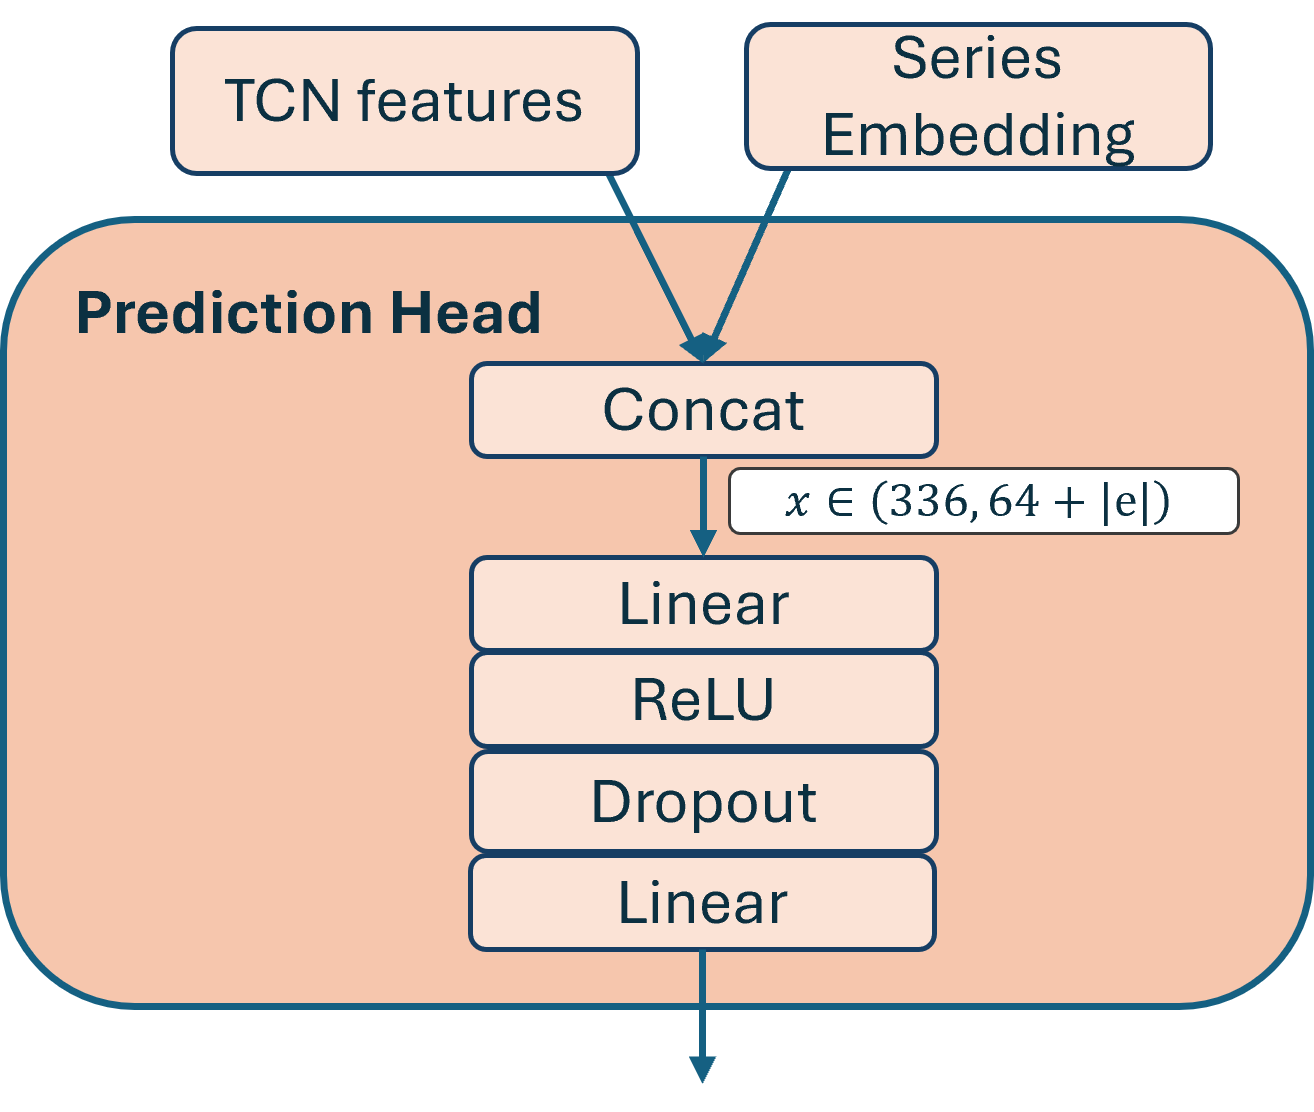
\includegraphics[width=\linewidth,height=0.52\textheight,keepaspectratio]{../../figures/pred_head_tcn.png}
        \caption{Prediction head with series conditioning.}
        \label{fig:tcn-prediction-head}
    \end{subfigure}
    \caption{Architecture of the proposed single-shot TCN forecaster. The complete model in (a) combines the 168-step history with known future covariates, processes the resulting sequence with seven dilated residual blocks, and predicts corrections to a repeated 24-hour seasonal baseline for the 336-step forecast horizon. Panel (b) shows the two normalized causal-convolution stages and skip connection within each residual block. Panel (c) shows how the prediction head concatenates the TCN features with a learned series embedding before producing the forecast correction.}
    \label{fig:tcn-architecture}
\end{figure}

\bibliographystyle{plain}
\bibliography{references}

\end{document}
